

\tikzset{every picture/.style={line width=0.75pt}} %set default line width to 0.75pt        

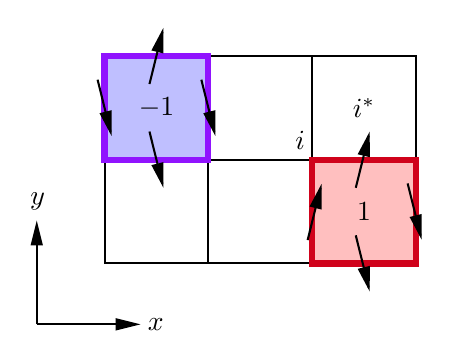
\begin{tikzpicture}[x=0.75pt,y=0.75pt,yscale=-1,xscale=1]
%uncomment if require: \path (0,300); %set diagram left start at 0, and has height of 300

%Shape: Square [id:dp4522225054629818] 
\draw  [fill={rgb, 255:red, 255; green, 0; blue, 0 }  ,fill opacity=0.25 ] (268,149) -- (318,149) -- (318,199) -- (268,199) -- cycle ;
%Shape: Square [id:dp4594732045911669] 
\draw  [fill={rgb, 255:red, 0; green, 0; blue, 255 }  ,fill opacity=0.25 ] (168,99) -- (218,99) -- (218,149) -- (168,149) -- cycle ;
%Straight Lines [id:da7859210255370197] 
\draw    (168,99) -- (218,99) ;
%Straight Lines [id:da12886428106250913] 
\draw    (168,149) -- (218,149) ;
%Straight Lines [id:da5836673303401485] 
\draw    (168,149) -- (168,99) ;
%Straight Lines [id:da6832798720040101] 
\draw    (218,149) -- (218,99) ;
%Shape: Square [id:dp4552383640295201] 
\draw   (168,99) -- (218,99) -- (218,149) -- (168,149) -- cycle ;
%Shape: Square [id:dp4299395977342566] 
\draw   (218,99) -- (268,99) -- (268,149) -- (218,149) -- cycle ;
%Shape: Square [id:dp7609749847711793] 
\draw   (218,149) -- (268,149) -- (268,199) -- (218,199) -- cycle ;
%Shape: Square [id:dp7189104654045673] 
\draw   (268,149) -- (318,149) -- (318,199) -- (268,199) -- cycle ;
%Shape: Square [id:dp3279496623171845] 
\draw   (168,149) -- (218,149) -- (218,199) -- (168,199) -- cycle ;
%Shape: Square [id:dp09533953088675018] 
\draw   (268,99) -- (318,99) -- (318,149) -- (268,149) -- cycle ;
%Shape: Square [id:dp6743217671924511] 
\draw  [color={rgb, 255:red, 144; green, 19; blue, 254 }  ,draw opacity=1 ][line width=2.25]  (168,99) -- (218,99) -- (218,149) -- (168,149) -- cycle ;
%Straight Lines [id:da23601359728908688] 
\draw [color={rgb, 255:red, 0; green, 0; blue, 0 }  ,draw opacity=1 ]   (189.64,112.54) -- (195.88,87.4) ;
\draw [shift={(196.36,85.46)}, rotate = 463.92] [fill={rgb, 255:red, 0; green, 0; blue, 0 }  ,fill opacity=1 ][line width=0.08]  [draw opacity=0] (12,-3) -- (0,0) -- (12,3) -- cycle    ;
%Straight Lines [id:da8963244134502486] 
\draw [color={rgb, 255:red, 0; green, 0; blue, 0 }  ,draw opacity=1 ]   (164.64,110.46) -- (170.88,135.6) ;
\draw [shift={(171.36,137.54)}, rotate = 256.08] [fill={rgb, 255:red, 0; green, 0; blue, 0 }  ,fill opacity=1 ][line width=0.08]  [draw opacity=0] (12,-3) -- (0,0) -- (12,3) -- cycle    ;
%Straight Lines [id:da6667388980914568] 
\draw [color={rgb, 255:red, 0; green, 0; blue, 0 }  ,draw opacity=1 ]   (189.64,135.46) -- (195.88,160.6) ;
\draw [shift={(196.36,162.54)}, rotate = 256.08] [fill={rgb, 255:red, 0; green, 0; blue, 0 }  ,fill opacity=1 ][line width=0.08]  [draw opacity=0] (12,-3) -- (0,0) -- (12,3) -- cycle    ;
%Straight Lines [id:da015522846808282864] 
\draw [color={rgb, 255:red, 0; green, 0; blue, 0 }  ,draw opacity=1 ]   (214.64,110.46) -- (220.88,135.6) ;
\draw [shift={(221.36,137.54)}, rotate = 256.08] [fill={rgb, 255:red, 0; green, 0; blue, 0 }  ,fill opacity=1 ][line width=0.08]  [draw opacity=0] (12,-3) -- (0,0) -- (12,3) -- cycle    ;
%Shape: Square [id:dp05679192513289277] 
\draw  [color={rgb, 255:red, 208; green, 2; blue, 27 }  ,draw opacity=1 ][line width=2.25]  (268,149) -- (318,149) -- (318,199) -- (268,199) -- cycle ;
%Straight Lines [id:da21391036278901998] 
\draw [color={rgb, 255:red, 0; green, 0; blue, 0 }  ,draw opacity=1 ]   (289.04,162.54) -- (295.28,137.4) ;
\draw [shift={(295.76,135.46)}, rotate = 463.92] [fill={rgb, 255:red, 0; green, 0; blue, 0 }  ,fill opacity=1 ][line width=0.08]  [draw opacity=0] (12,-3) -- (0,0) -- (12,3) -- cycle    ;
%Straight Lines [id:da9816247930379984] 
\draw [color={rgb, 255:red, 0; green, 0; blue, 0 }  ,draw opacity=1 ]   (289.04,185.46) -- (295.28,210.6) ;
\draw [shift={(295.76,212.54)}, rotate = 256.08] [fill={rgb, 255:red, 0; green, 0; blue, 0 }  ,fill opacity=1 ][line width=0.08]  [draw opacity=0] (12,-3) -- (0,0) -- (12,3) -- cycle    ;
%Straight Lines [id:da31464719110814876] 
\draw [color={rgb, 255:red, 0; green, 0; blue, 0 }  ,draw opacity=1 ]   (314.04,160.46) -- (320.28,185.6) ;
\draw [shift={(320.76,187.54)}, rotate = 256.08] [fill={rgb, 255:red, 0; green, 0; blue, 0 }  ,fill opacity=1 ][line width=0.08]  [draw opacity=0] (12,-3) -- (0,0) -- (12,3) -- cycle    ;
%Straight Lines [id:da8559300619509063] 
\draw [color={rgb, 255:red, 0; green, 0; blue, 0 }  ,draw opacity=1 ]   (265.84,187.74) -- (272.08,162.6) ;
\draw [shift={(272.56,160.66)}, rotate = 463.92] [fill={rgb, 255:red, 0; green, 0; blue, 0 }  ,fill opacity=1 ][line width=0.08]  [draw opacity=0] (12,-3) -- (0,0) -- (12,3) -- cycle    ;
%Straight Lines [id:da015254394235462598] 
\draw    (135.33,228.33) -- (183.33,228.33) ;
\draw [shift={(185.33,228.33)}, rotate = 180] [fill={rgb, 255:red, 0; green, 0; blue, 0 }  ][line width=0.08]  [draw opacity=0] (12,-3) -- (0,0) -- (12,3) -- cycle    ;
%Straight Lines [id:da5713451115525661] 
\draw    (135.33,228.33) -- (135.33,180.33) ;
\draw [shift={(135.33,178.33)}, rotate = 450] [fill={rgb, 255:red, 0; green, 0; blue, 0 }  ][line width=0.08]  [draw opacity=0] (12,-3) -- (0,0) -- (12,3) -- cycle    ;

% Text Node
\draw (193,124) node    {$-1$};
% Text Node
\draw (293,174) node    {$1$};
% Text Node
\draw (293,124) node    {$\boldsymbol{i}^{*}$};
% Text Node
\draw (266,145.6) node [anchor=south east] [inner sep=0.75pt]    {$\boldsymbol{i}$};
% Text Node
\draw (187.33,228.33) node [anchor=west] [inner sep=0.75pt]    {$x$};
% Text Node
\draw (135.45,174.94) node [anchor=south] [inner sep=0.75pt]  [rotate=-2]  {$y$};


\end{tikzpicture}
